\section{Que es la regresión lineal múltiple}


\section{Metodología}
Usamos las siguientes importaciones para el programa
\begin{figure}[h]
    \centering
    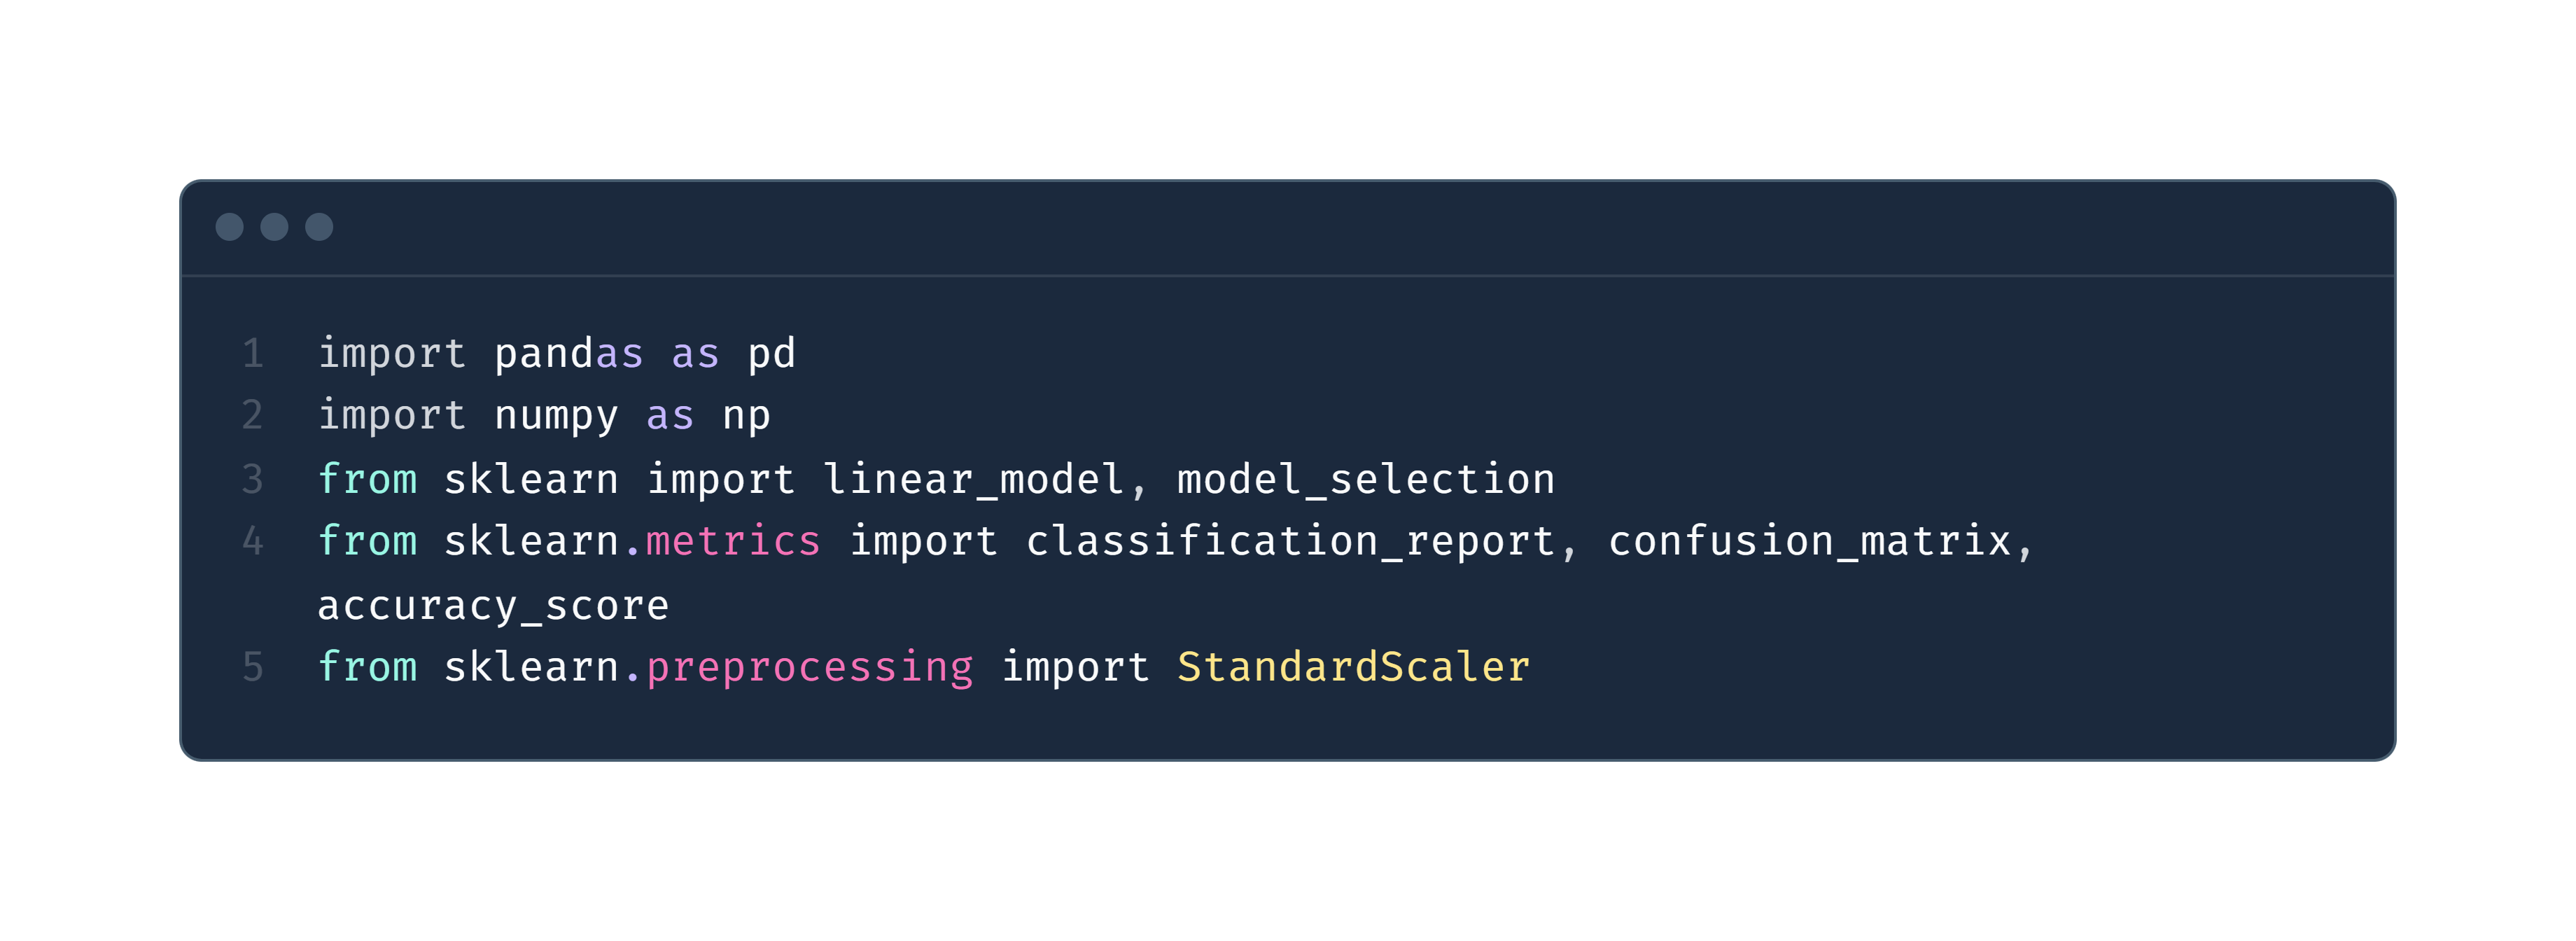
\includegraphics[width=0.5\linewidth]{image.png}
\end{figure}
El codigo del programa es el siguiente:
\begin{figure}[h]
    \centering
    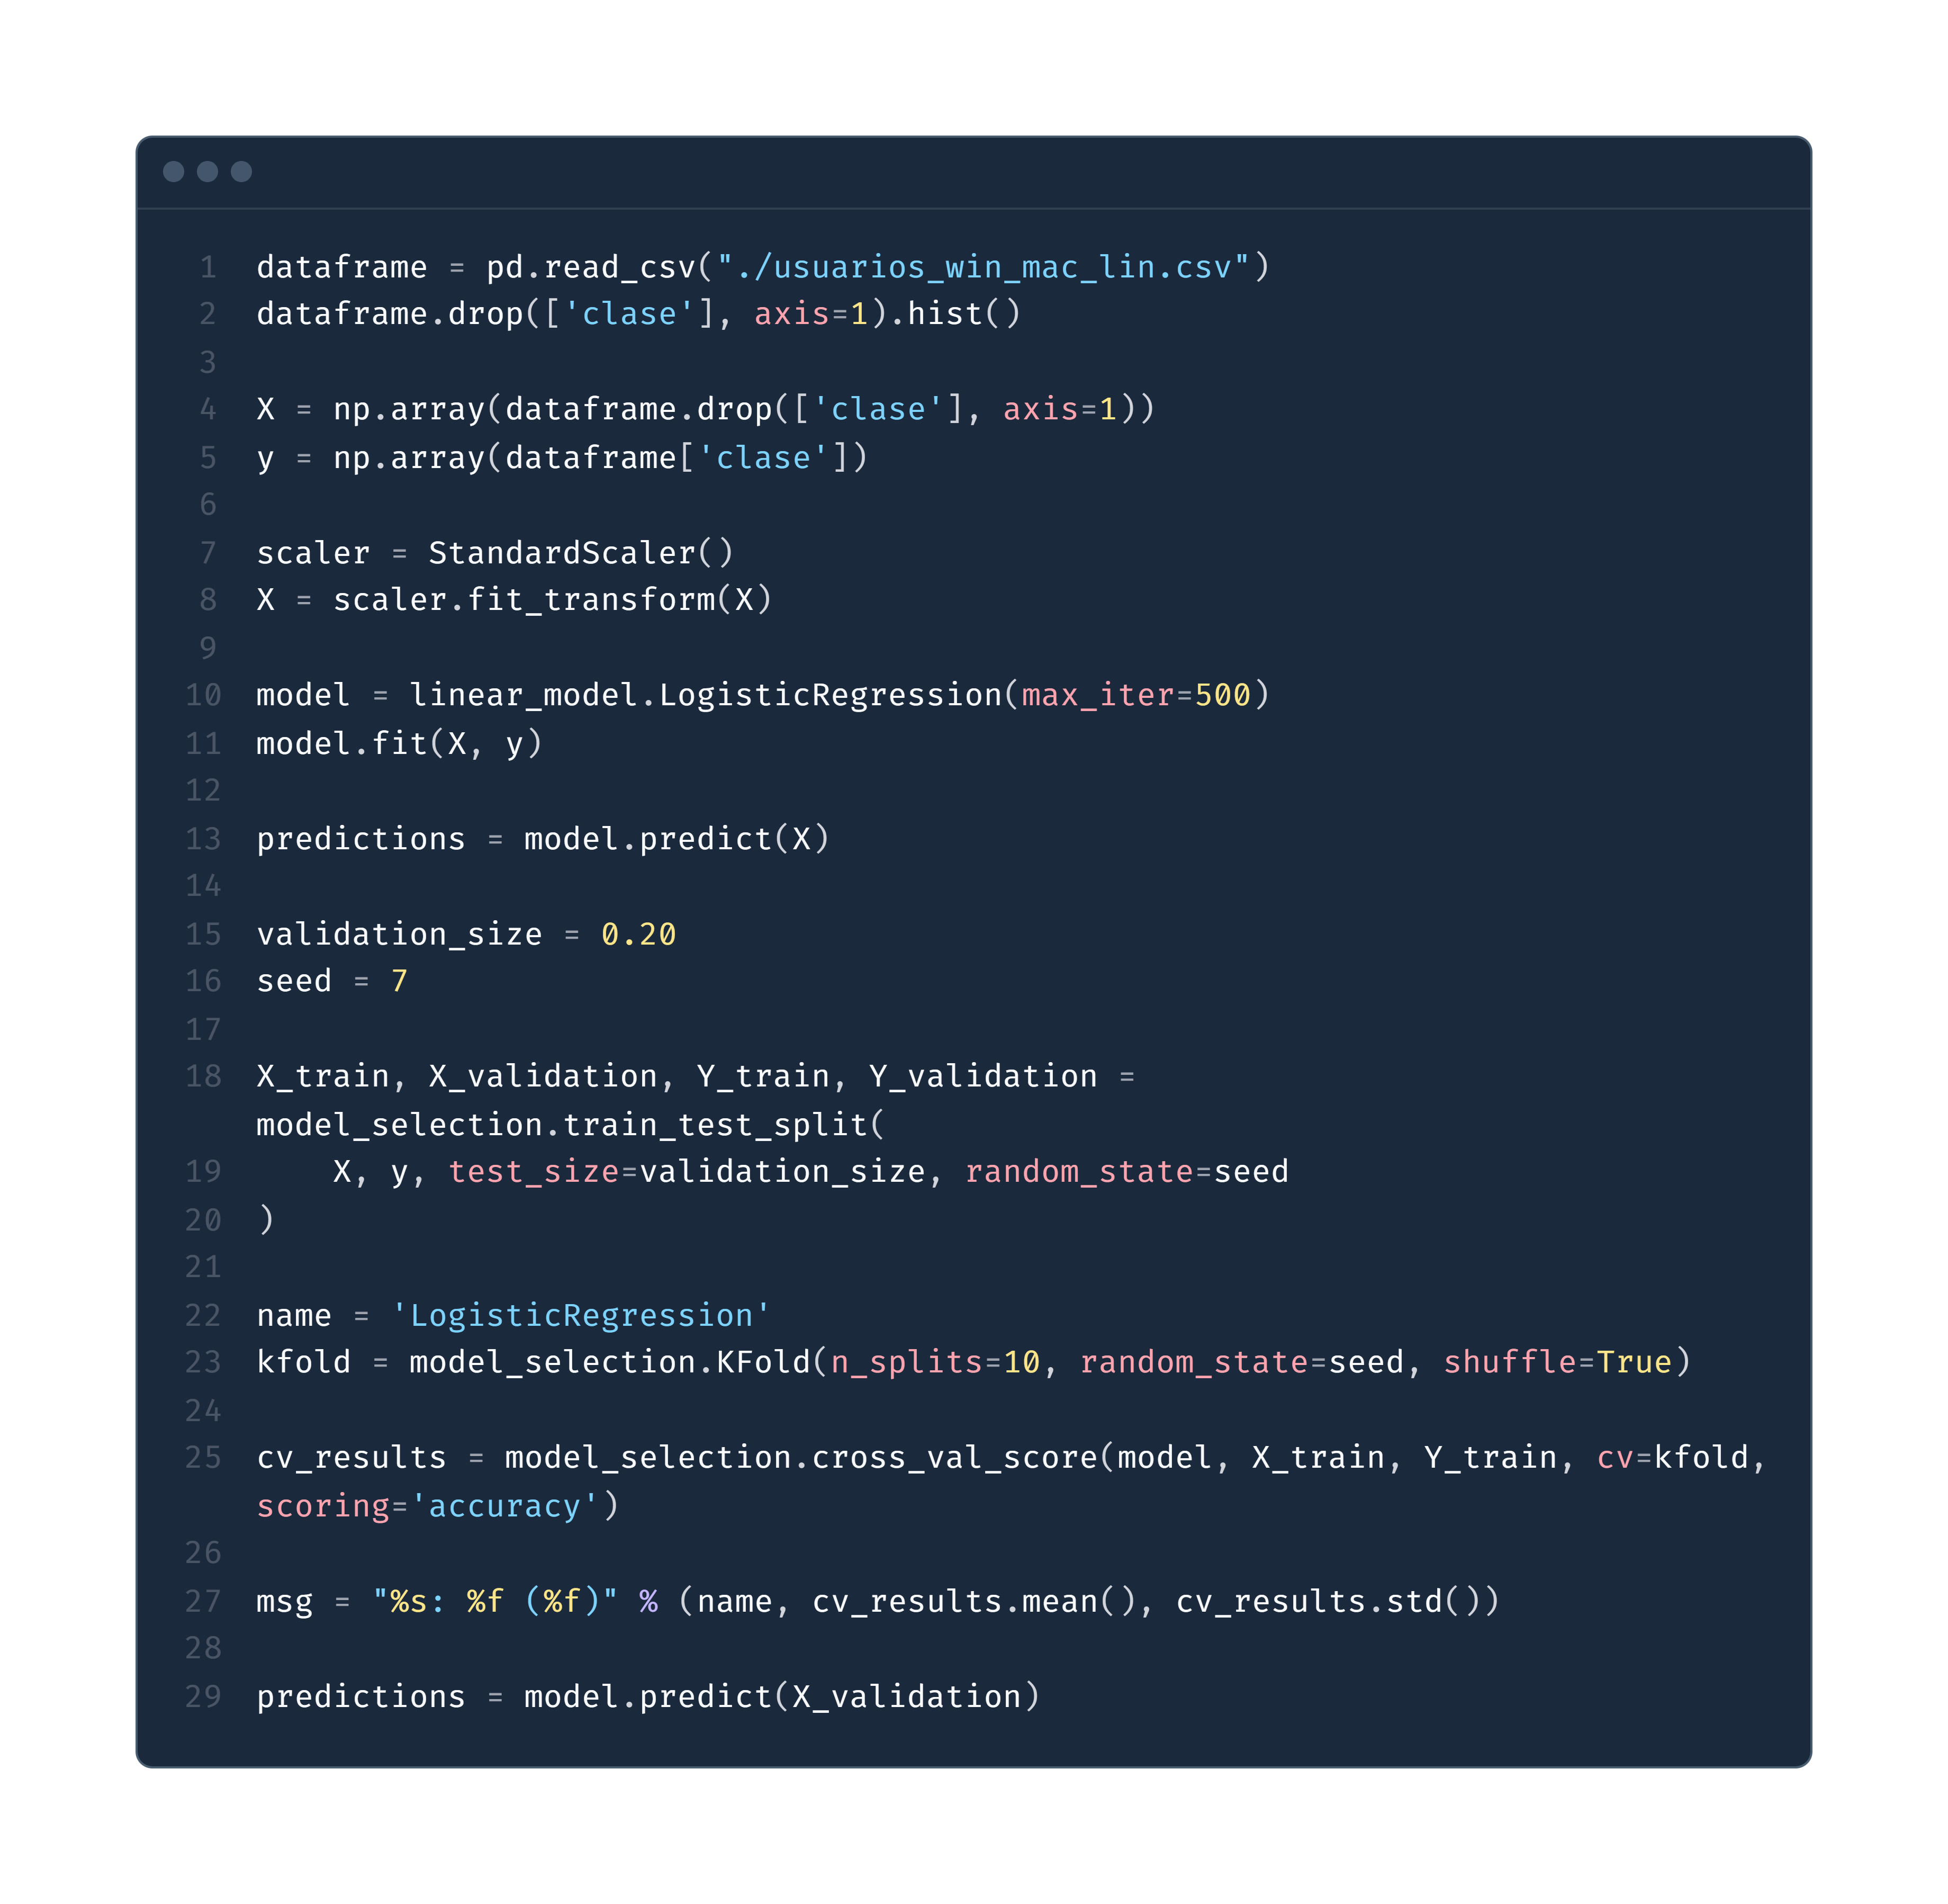
\includegraphics[width=0.5\linewidth]{image_2.png}
\end{figure}

se modifico algunas partes del código ya que había elementos obsoletos que hacían que el programa no funcionara.
Por ejemplo, en la linea de codigo "dataframe.drop(['clase'], 1) " era necesario remplazar por dataframe.drop(['clase'], axis=1) 
en la linea "kfold=model\_selection.KFold(n\_splits=10,random\_state=seed) " era necesario agregar  un shuffle=True


\section{Resultados}
Al ejecutar el programa obtenemos los siguientes valores
Dimensiones de X: ($170$, $4$)
Primeras $0$ predicciones: [$2$ $2$ $2$ $2$ $0$]
Precisión en datos de entrenamiento: $0.7$
LogisticRegression: $0.630769$ ($0.136055$)
Precisión en datos de validación: $0.7352941176470589$
Matriz de confusion
A = 
$$\begin{bmatrix}
14 & 0 & 4 \\
4 & 2 & 0 \\
1 & 0 & 9
\end{bmatrix}$$

Reporte de clasificación:
\begin{table}[h]
    \centering
    \begin{tabular}{lcccc}
        \toprule
        \textbf{Clase} & \textbf{Precisión} & \textbf{Recall} & \textbf{F1-Score} & \textbf{Soporte} \\
        \midrule
        0 & 0.74 & 0.78 & 0.76 & 18 \\
        1 & 1.00 & 0.33 & 0.50 & 6 \\
        2 & 0.69 & 0.90 & 0.78 & 10 \\
        \midrule
        \multicolumn{3}{l}{\textbf{Exactitud}} & 0.74 & 34 \\
        \midrule
        \textbf{Promedio macro} & 0.81 & 0.67 & 0.68 & 34 \\
        \textbf{Promedio ponderado} & 0.77 & 0.74 & 0.72 & 34 \\
        \bottomrule
    \end{tabular}
    \caption{Reporte de clasificación}
    \label{tab:reporte_clasificacion}
\end{table}
\section{Conclusión}
El modelo tiene un buen nivel de prediccion ($70\%$), aun que puede ser mejorable, ya tendrá buenas predicciones, podría mejorarse aumentando la cantidad de datos en la clase 1 ya que tiene un porcentaje de recall muy bajo, el modelo solo predice un clase 1 cuando este realmente seguro.